% enable this to activate the version for PRINT
% disable this to make the pdf symmetric and without white pages
% => asymmetric alternating left/right margins
% \newcommand*{\printversion}{}%

%% | ---------------- document meta information --------------- |

\newcommand{\Author}{John Smith}
\newcommand{\Department}{Department of Cybernetics}
\newcommand{\Supervisor}{Ing. My Supervisor, Ph.D.}
\newcommand{\SupervisorSpecialist}{Ing. My Specialist, Ph.D.}
\newcommand{\Programme}{Electrical Engineering and Information Technology}
\newcommand{\Field}{Artificial Intelligence and Biocybernetics}
\newcommand{\Title}{My Thesis Title\\[0.5em]Can Span Multiple Lines}
\newcommand{\Keywords}{Unmanned Aerial Vehicles, Automatic Control}
\newcommand{\KlicovaSlova}{Bezpilotní Prostředky, Automatické Řízení}
\newcommand{\Year}{2021}
\newcommand{\Month}{January}
\newcommand{\Date}{\Month~\Year}
\newcommand{\Location}{Prague}

%% | ---------------------- configuration --------------------- |

% most of the configuration stuff happens here
%!TEX root = ../main.tex

%% | ----------------------- page setup ----------------------- |

% define documentclass based on the print/screen version of the document
\pdfoutput=1
\ifdefined\printversion
  \documentclass[a4paper,11pt,twoside,openright]{book}
\else
  \documentclass[a4paper,11pt,twoside,openany]{book}
\fi

% define how "clearpage" works with the print/screen version of the document
\newcommand{\conditionalClearPage}{
  \ifdefined\printversion
    \cleardoublepage
  \else
    \clearpage
  \fi
}

%% | ----------------- commonly used packages ----------------- |

\usepackage[english]{babel}
\usepackage[utf8]{inputenc}
\usepackage{csquotes}
\usepackage{amsmath,amsfonts,amssymb,bm}
\usepackage{nicefrac}
\usepackage{algorithm,algpseudocode}
\usepackage[title,titletoc]{appendix}
\usepackage{latexsym}
\usepackage{a4wide}
\usepackage{color}
\usepackage{indentfirst}
\usepackage{graphicx}
\usepackage{fancyhdr,lastpage}
\usepackage{longtable}
\usepackage{pifont}
\usepackage{makeidx}
\usepackage{multirow}
\usepackage{dcolumn}
\usepackage{epstopdf}
\usepackage{url}
\usepackage{listings}
\usepackage{relsize}
\usepackage{pdfpages}
\usepackage{url}
\usepackage{lipsum}
\usepackage{isotope}
\usepackage{verbatim}
\usepackage{xcolor}
\usepackage{tcolorbox}
\usepackage[colorlinks]{hyperref}
\usepackage{multicol}
\usepackage{subfig}
\usepackage[export]{adjustbox}

\usepackage{svg}

% print version has different margins to accommodate the spine of the book
% do not move this around, or it stops working
\ifdefined\printversion
  \usepackage[a4paper,margin=3.2cm,inner=3.4cm,outer=2.0cm]{geometry}
\else
  \usepackage[a4paper,margin=3.2cm,inner=2.7cm,outer=2.7cm]{geometry}
\fi

\hyphenation{}

%% | --------------------- custom commands -------------------- |

\definecolor{cvutblue}{cmyk}{1, 0.43, 0, 0}

% set itemize: bullets type and color
\renewcommand{\labelitemi}{\textcolor{cvutblue}{\raisebox{.45ex}{\rule{.8ex}{.8ex}}}}
\renewcommand{\labelitemii}{\textcolor{cvutblue}{\raisebox{.45ex}{\rule{.8ex}{.8ex}}}}
\renewcommand{\labelitemiii}{\textcolor{cvutblue}{\raisebox{.45ex}{\rule{.8ex}{.8ex}}}}
\renewcommand{\labelitemiv}{\textcolor{cvutblue}{\raisebox{.45ex}{\rule{.8ex}{.8ex}}}}


%% | ---------------------- abbreviations --------------------- |

\usepackage[printonlyused]{acronym}

% use to change margins around abbreviations block
\def\changemargin#1#2{\list{}{\rightmargin#2\leftmargin#1}\item[]}
\let\endchangemargin=\endlist

%% | -------------------- hyper links setup ------------------- |
\hypersetup{
  linkcolor=black,
  anchorcolor=black,
  citecolor=cvutblue,
  filecolor=black,
  menucolor=black,
  runcolor=black,
  urlcolor=cvutblue
}


%% | -------------------------- tikz -------------------------- |

\usepackage{tikz}
\usepackage{pgfplots}
\pgfplotsset{compat=1.14}
\usetikzlibrary{backgrounds,arrows,automata,shapes,positioning,calc,through,spy,shapes,shapes.geometric,shapes.multipart,fit,patterns,fadings}
\pgfdeclarelayer{background}
\pgfdeclarelayer{foreground}
\pgfsetlayers{background,main,foreground}

%% | ------------ siunitx for units of measurements ----------- |

\usepackage{siunitx}
\DeclareSIUnit \parsec {pc}
\DeclareSIUnit \electronvolt {eV}
\DeclareSIUnit \pixel {px}
\DeclareSIUnit \arcmin {arcmin}
\DeclareSIUnit \erg {erg}
\DeclareSIUnit \joul {J}

%% | --------------- change formatting of lists --------------- |

\usepackage{enumitem}
\setlist{nosep}

\renewcommand{\labelenumi}{(\roman{enumi})}

%% | -------------------- table of contents ------------------- |

\usepackage[subfigure]{tocloft}

\tocloftpagestyle{plain}

%% | ----------------- formatting of a chapter ---------------- |

\usepackage{titlesec}

\titleformat{\chapter}[hang]{}{\color{cvutblue}\rule[-0.03cm]{0.50cm}{0.50cm}}{3.2\parskip}{\normalfont\bfseries\LARGE\thechapter\hspace{0.5cm}}
\titlespacing*{\chapter}{0pt}{-1em}{1.5em}

%% | ----------------- formatting of a section ---------------- |

\titleformat{\section}[hang]{}{\hspace{0.11cm}\color{cvutblue}\rule[-0.02cm]{0.30cm}{0.30cm}}{3.7\parskip}{\normalfont\bfseries\large\thesection\hspace{0.5cm}}
\titlespacing*{\section}{0pt}{1em}{0.5em}

\titleformat{name=\section,numberless}[block]
{\normalfont\large\bfseries}{}{0pt}{\large}
% {?}{before}{after}
\titlespacing*{name=\section,numberless}{0pt}{-1em}{2em}

%% | --------------- formatting of a subsection --------------- |

\titleformat{\subsection}[hang]{}{\hspace{0.16cm}\color{cvutblue}\rule[0.03cm]{0.20cm}{0.20cm}}{4.0\parskip}{\normalfont\bfseries\normalsize}
\titlespacing*{\subsection}{0pt}{1em}{0.5em}



%% | ------------------------ biblatex ------------------------ |

% \usepackage[backend=bibtex,defernumbers=true,style=ieee,sorting=ydnt,sortcites=true]{biblatex}
\usepackage[backend=bibtex,defernumbers=true,style=ieee,sorting=none,sortcites=true]{biblatex}

% define the source file with bibliography
\addbibresource{main.bib}

\renewcommand*{\bibfont}{\Font}

% add suffix "a" to publications containing the keyword "mine"
% add suffix "c" to publications containing the keyword "mine" && "core"
\DeclareFieldFormat{labelnumber}{%
  \ifkeyword{mine}
    {\ifkeyword{core}
      {{\number\numexpr#1}c}%
      {{\number\numexpr#1}a}%
    }%
    {#1}%
}

\DeclareCiteCommand{\tabcite}%[\mkbibbrackets]
  {\usebibmacro{cite:init}%
   \usebibmacro{prenote}}
  {\usebibmacro{citeindex}%
   \usebibmacro{cite:comp}}
  {}
  {\usebibmacro{cite:dump}%
   \usebibmacro{postnote}}

% define fullciteinbox command
\definecolor{light-gray}{gray}{0.95}
\newcommand{\fullciteinbox}[2]{%

\DeclareCiteCommand{\fullcite}
{\usebibmacro{prenote}}
{\clearfield{addendum}%
  \usedriver
  {\defcounter{minnames}{6}%
  \defcounter{maxnames}{6}}
{\thefield{entrytype}}}
{\multicitedelim}
{\usebibmacro{postnote}}

\begin{tcolorbox}[opacityfill=0.05,width=\textwidth,colback={cvutblue},colframe={cvutblue},title={}]%
\ifx&#2&
\else
  \textbf{#2}:\\\\
\fi
\begin{minipage}[t]{0.07\linewidth}%
\raggedright%
\cite{#1}%
\end{minipage}%
\begin{minipage}[t]{0.93\linewidth}%
\fullcite{#1}%
\end{minipage}%
\end{tcolorbox}%
%}%
\vspace{-0.3em}
}%

% change the bibliography font style
% does not compile without this
\let\bibfont\small

% this is used to print citations of author's work
\defbibenvironment{mycitations}
{\itemize}
{\enditemize}
{\item}

%% | ---------------------- custom macros --------------------- |

\newcommand{\strong}[1]{\textbf{#1}}
\newcommand{\coord}[1]{\textbf{#1}}
\newcommand{\norm}[1]{\left\lvert#1\right\rvert}
\newcommand{\m}[1]{\ensuremath{\mathbf{#1}}}
\newcommand\numberthis{\addtocounter{equation}{1}\tag{\theequation}}
\newcommand{\add}[1]{{\color{green} {#1}}}
\newcommand{\todo}[1]{{\color{red} TODO {#1}}}
\newcommand{\updated}[1]{{\color{blue} {#1}}}
\newcommand{\real}{\mathbb{R}}
\newcommand{\red}[1]{{\color{red} #1}}
\newcommand{\minus}{\scalebox{0.75}[1.0]{$-$}}
\newcommand{\plus}{\scalebox{0.8}[0.8]{$+$}}
\newcommand{\figvspace}{\vspace{-1em}}

% referencing
\newcommand{\reffig}[1]{Fig.~\ref{#1}}
\newcommand{\reflst}[1]{Lst.~\ref{#1}}
\newcommand{\refalg}[1]{Alg.~\ref{#1}}
\newcommand{\refsec}[1]{Sec.~\ref{#1}}
\newcommand{\reftab}[1]{Table~\ref{#1}}
\newcommand{\refeq}[1]{\eqref{#1}}

%% | ----------------- listings - showing code ---------------- |

\usepackage{listings}     
\usepackage{lstautogobble}  % Fix relative indenting
\usepackage{color}          % Code coloring
\usepackage{zi4}            % Nice font

\definecolor{bluekeywords}{rgb}{0.13, 0.13, 1}
\definecolor{greencomments}{rgb}{0, 0.5, 0}
\definecolor{redstrings}{rgb}{0.9, 0, 0}
\definecolor{graynumbers}{rgb}{0.5, 0.5, 0.5}

\usepackage{listings}
\lstset{
    autogobble,
    columns=fullflexible,
    showspaces=false,
    showtabs=false,
    breaklines=true,
    showstringspaces=false,
    breakatwhitespace=true,
    escapeinside={(*@}{@*)},
    commentstyle=\color{greencomments},
    keywordstyle=\color{bluekeywords},
    stringstyle=\color{redstrings},
    numberstyle=\color{graynumbers},
    basicstyle=\ttfamily\footnotesize,
    frame=l,
    framesep=12pt,
    xleftmargin=12pt,
    tabsize=4,
    captionpos=b
}

%% | -------------------- layout parameters ------------------- |

% no indent, free space between paragraphs
\setlength{\parindent}{1cm}
\setlength{\parskip}{1ex plus 0.5ex minus 0.2ex}

% offsets the head down
\setlength{\headheight}{18pt}

% foot line
\renewcommand{\footrulewidth}{0.4pt}

%% | -------------- define the 'full' page style -------------- |

\fancypagestyle{full}{%
  % \fancyhf{} % This is a more concise way to clear everything
  % \renewcommand{\headrulewidth}{0.4pt} % Or your preferred value for the header rule
  % \renewcommand{\footrulewidth}{0pt}   % No rule for the footer, or set as desired

  \fancyhead[LO]{\leftmark}
  \fancyhead[RE]{\rightmark}


  \fancyfoot[LO]{\thepage/\pageref{LastPage}} % Page number on the Left
  \fancyfoot[RO]{CTU in Prague}             % "CTU in Prague" on the Right

  \fancyfoot[LE]{CTU in Prague}             % "CTU in Prague" on the Left
  \fancyfoot[RE]{\thepage/\pageref{LastPage}} % Page number on the Right

  % \fancyfoot[C]{} % You can add this for explicitness if you wish
}




% \fancypagestyle{full}{%

%   % clear the default layout
%   \fancyhead{}
%   \fancyfoot{}

%   % page header
%   \fancyhead[LO]{\leftmark}
%   \fancyhead[RE]{\rightmark}
%   \fancyhead[LE,RO]{\thepage/\pageref{LastPage}}

%   % page footer
%   \fancyfoot[L]{CTU in Prague}
%   \fancyfoot[R]{\Department}
%   \fancyfoot[C]{}
% }

%% | -------------- define the 'plain' page style ------------- |

\fancypagestyle{plain}{%

  % clear the default layout
  \fancyhead{}
  \fancyfoot{}

  % page header
  % \fancyhead[LE,RO]{\thepage}
}

%% | -------------- Adjust style of chapter names ------------- |

\renewcommand{\chaptermark}[1]{\markboth{\MakeUppercase{\thechapter.\ #1}}{}}

%% | -------- European layout, no extra space after '.' ------- |

\frenchspacing

%% | ----------- adjust the style of the first page ----------- |

\makeatletter
\renewcommand\chapter{\if@openright\cleardoublepage\else\clearpage\fi
                    \thispagestyle{full}% original style: plain
                    \global\@topnum\z@
                    \@afterindentfalse
                    \secdef\@chapter\@schapter}
\makeatother


%% | ---------------------- the contents ---------------------- |

\begin{document}

% this will prevent unwanted line overflows
% http://latexref.xyz/_005cfussy-_0026-_005csloppy.html
\sloppy

\pagenumbering{roman}

%% --------------------------------------------------------------
%% |                         Title page                         |
%% --------------------------------------------------------------

%!TEX root = ../main.tex

\begin{titlepage}
  \begin{center}

    \textsc{\Large Czech Technical University in Prague}\\[1em]
    \textsc{\large Faculty of Electrical Engineering\\
    \Department\\
    Multi-robot Systems\\[3em]
    }
    
\includegraphics[height=4.1cm]{fig/ctu_lion.pdf}\\[3em]

    \textbf{\textsc{\Huge \Title}}\\[2em]

    \textbf{\Large Bachelor's Thesis}\\[6em]

    \textbf{\huge \Author}\\[6em]

    {\large \Location, \Date}\\[3em]

    Study programme: \Programme\\
    Branch of study: \Field\\[4em]

    \textbf{Supervisor: \Supervisor}\\

    \vspace{2pt}

  \end{center}
\end{titlepage}


% set up the page style for the "intro" pages
\pagestyle{plain}

%% --------------------------------------------------------------
%% |                       Acknowledgments                      |
%% --------------------------------------------------------------

\conditionalClearPage

%!TEX root = ../main.tex

\section*{Acknowledgments}

I would like to express my sincere gratitude to my supervisor, MSc. Manuel Boldrer, Ph.D., for his valuable guidance, helpful feedback, and for providing direction throughout the development of this thesis. 
His expertise was irreplaceable in shaping this work.

My appreciation also extends to the members of the Multi-robot Systems (MRS) group. 
I am particularly grateful for their support and practical assistance during the experimental phase, especially concerning safety during experiments and for helping me understand various technical aspects. 
Their willingness to share knowledge was very beneficial.

Finally, I would like to extend my thanks to my family for their support, patience, and encouragement throughout my studies and the writing of this thesis. 
Their belief in me has been a constant source of motivation.

\vspace{2.5cm}


%% --------------------------------------------------------------
%% |                         Assignment                         |
%% --------------------------------------------------------------

\conditionalClearPage

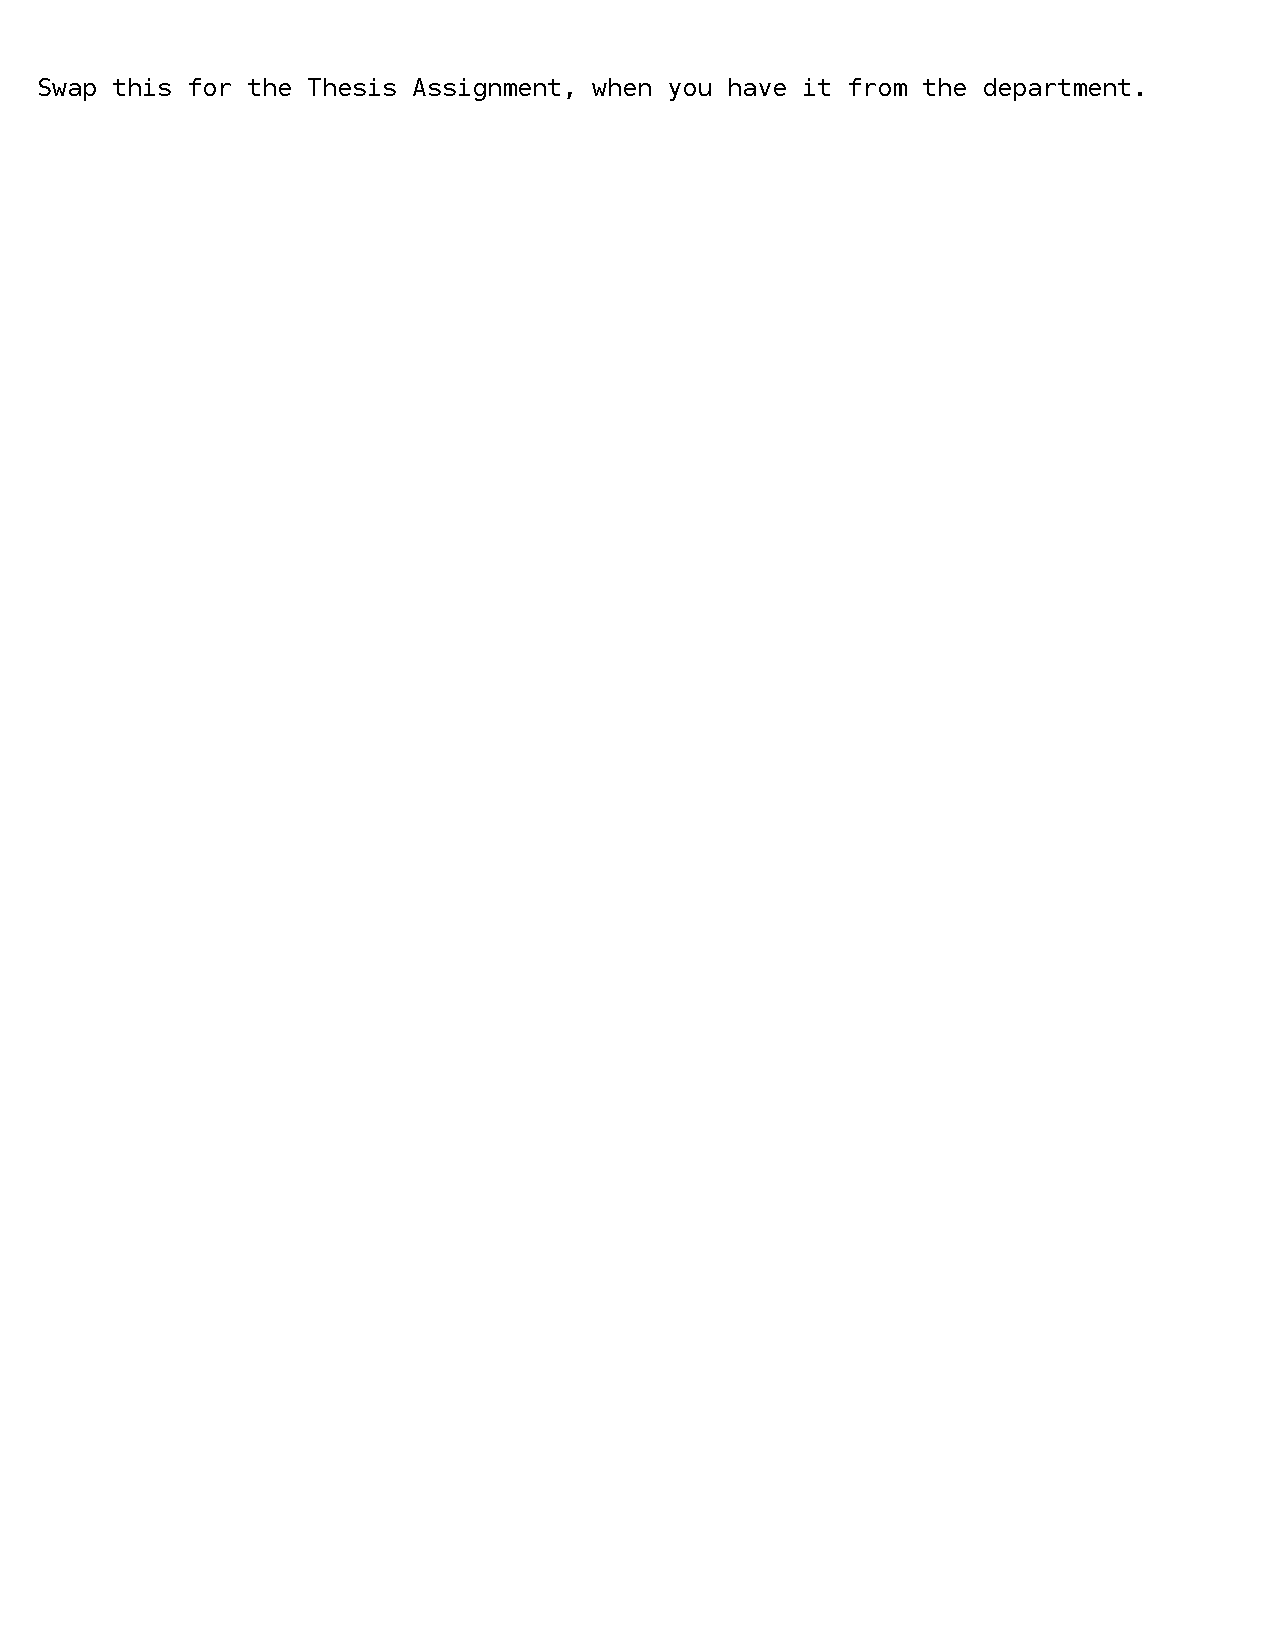
\includepdf{src/assignment.pdf}

%% --------------------------------------------------------------
%% |                         Declaration                        |
%% --------------------------------------------------------------

\conditionalClearPage

~\vfill{}

\section*{Declaration}
%\section*{Prohlášení autora práce}

I declare that presented work was developed independently, and that I have listed all sources of information used within, in accordance with the Methodical instructions for ob-serving ethical principles in preparation of university theses.
% Prohlašuji, že jsem předloženou práci vypracoval samostatně a že jsem uvedl veškeré použité informační zdroje v souladu s Metodickým pokynem o dodržování etických principů při přípravě vysokoškolských závěrečných prací.

\vspace{1.5cm}
~\\

Date .............................\hfill{}...............................................
% Dne.............................\hfill{}...............................................

\hfill{}~~~~~~~~~~~~~~~

\newpage{}


%% --------------------------------------------------------------
%% |                          Abstracts                         |
%% --------------------------------------------------------------

\conditionalClearPage

%!TEX root = ../main.tex

\begin{changemargin}{0.8cm}{0.8cm}

~\vfill{}

\section*{Abstract}
\vskip 0.5em

% Achieving effective multi-agent \ac{UAV} coordination without explicit communication, alongside robust single-agent navigation in complex, \ac{GNSS}-denied environments, presents significant research challenges.
% Therefore, developing robust algorithms capable of handling these demanding conditions is necessary.
% This thesis addresses these challenges through two primary objectives. 
% The first objective is to extend the \ac{RBL} algorithm for multi-agent coordination from two to three dimensions, introducing new rules for enhanced performance. 
% The second objective involves implementing and validating this 3D \ac{RBL} framework for single \ac{UAV} navigation in a real-world forest environment using \ac{LiDAR} sensing.

% The 2D \ac{RBL} algorithm was extended to 3D by building upon its foundational concepts and introducing new rules for vertical control. 
% For single-agent forest navigation, this 3D \ac{RBL} was integrated with \ac{LiDAR}-based perception, utilizing Point-LIO for state estimation and a voxel-based mapping approach. 
% The system was evaluated through multi-agent simulations and real-world flight experiments in a forest.

% Simulations demonstrated the successful extension of \ac{RBL} to 3D, showing improved multi-agent coordination efficiency, particularly with more agents. 
% Real-world experiments validated the effectiveness of the implemented system for autonomous point-to-point navigation in a forest, though challenges with mapping dynamic environmental elements like leaves were identified as a limitation.

% In summary, this thesis validates the modification and real-world use of the \ac{RBL} algorithm for 3D \ac{UAV} point-to-point navigation.
% While the need for enhanced mapping is needed, the results of this study significantly contribute to the development of more independent and adaptable \ac{UAV} systems.

% The study of autonomous \acp{UAV} has become a prominent sub-field of mobile robotics.


\ac{UAVs} are increasingly transitioning from open-sky operations to complex, \ac{GNSS}-denied environments, presenting significant challenges for multi-agent coordination and single-agent autonomous navigation. 
This thesis addresses these issues by first extending the \ac{RBL} algorithm from two to three dimensions for multi-\ac{UAV} communication-free coordination.
New rules were developed to manage vertical movement and enhance 3D coordination efficiency. 
Secondly, the thesis investigates the practical application of this 3D \ac{RBL} for single \ac{UAV} navigation in a challenging forest environment, utilizing onboard \ac{LiDAR} sensing.

The methodology involved adapting the core \ac{RBL} for 3D space and integrating it with real-time perception systems. 
For the single-agent navigation task, this included \ac{LiDAR}-based point cloud processing, state estimation using Point-LIO, and voxel-based environmental mapping with Bonxai. 
Strategies to minimize limitations from anisotropic sensors, such as restricted \ac{LiDAR} \ac{FOV}, were also developed. 
The proposed algorithm was evaluated through extensive simulations in the multi-agent scenario and validated with real-world experiments in a forest environment for the single-agent case.
% The extended 3D \ac{RBL} was evaluated in simulated multi-agent coordination scenarios, while the integrated single-agent system was validated through real-world flight experiments in a forest.

Simulations confirmed the successful 3D extension of the \ac{RBL} algorithm, demonstrating effective multi-agent coordination. 
Real-world experiments validated the capability of the 3D \ac{RBL}-based system for autonomous point-to-point navigation in a forest. %, as illustrated in accompanying videos \cite{aggressive_flight}, \cite{conservative_flight}. 
However, limitations were identified, particularly in the mapping system's handling of dynamic environmental elements, which occasionally led to navigation failures.% \cite{flight_fail}.

% In conclusion, this thesis demonstrates the successful adaptation and practical application of the \ac{RBL} algorithm for 3D \ac{UAV} operations. 
% It contributes a 3D extension for multi-agent coordination and a validated system for single-agent navigation in complex, real-world settings, addressing challenges posed by sensor limitations. 
% While further work on robust mapping in dynamic environments is indicated, the findings provide a valuable foundation for advancing autonomous UAV systems.




\vskip 1em

{\bf Keywords} \Keywords

\vskip 2.5cm

\end{changemargin}


\conditionalClearPage

%!TEX root = ../main.tex

\begin{changemargin}{0.8cm}{0.8cm}

~\vfill{}

\section*{Abstrakt}
\vskip 0.5em

\sloppy
Výzkum na poli autonomních bezpilotních prostředků (UAV) se stal významným oborem mobilní robotiky.

\vskip 1em

{\bf Klíčová slova} \KlicovaSlova

\vskip 2.5cm

\end{changemargin}


%% --------------------------------------------------------------
%% |                        Abbreviations                       |
%% --------------------------------------------------------------

\conditionalClearPage

\begin{changemargin}{0.8cm}{0.8cm}

~\vfill{}

\section*{Abbreviations}

% this will print only the used abbreviations
%!TEX root = ../main.tex

\begin{acronym}
  \acro{API}[API]{Application Programming Interface}
  \acro{CTU}[CTU]{Czech Technical University}
  \acro{DOF}[DOF]{degree-of-freedom}
  \acro{FOV}[FOV]{Field of View}
  \acro{GNSS}[GNSS]{Global Navigation Satellite System}
  \acro{GPS}[GPS]{Global Positioning System}
  \acro{IMU}[IMU]{Inertial Measurement Unit}
  \acro{LKF}[LKF]{Linear Kalman Filter}
  \acro{LTI}[LTI]{Linear time-invariant}
  \acro{LiDAR}[LiDAR]{Light Detection and Ranging}
  \acro{MAV}[MAV]{Micro Aerial Vehicle}
  \acro{MPC}[MPC]{Model Predictive Control}
  \acro{MRS}[MRS]{Multi-robot Systems Group}
  \acro{ROS}[ROS]{Robot Operating System}
  \acro{RTK}[RTK]{Real-time Kinematics}
  \acro{SLAM}[SLAM]{Simultaneous Localization And Mapping}
  \acro{UAV}[UAV]{Unmanned Aerial Vehicle}
  \acro{UGV}[UGV]{Unmanned Ground Vehicle}
  \acro{UKF}[UKF]{Unscented Kalman Filter}
  \acro{RBL}[RBL]{Rule-based Lloyd Algorithm}
  \acro{ToF}[ToF]{Time-of-Flight}
  \acro{PCL}[PCL]{Point Cloud Library}
  \acro{GNSS}[GNSS]{Global Navigation Satellite System}
  \acro{3D}[3D]{three-dimensional}
  \acro{2D}[2D]{two-dimensional}
  \acro{EMI}[EMI]{Electromagnetic Interference}\
  \acro{IMU}[IMU]{Inertial Measurement Unit}
\end{acronym}


\vskip 2.5cm

\end{changemargin}

\conditionalClearPage

%% --------------------------------------------------------------
%% |                      Table of contents                     |
%% --------------------------------------------------------------

\tableofcontents

\conditionalClearPage

% set up the full page style with normal page numbering
\pagestyle{full}
\pagenumbering{arabic}

%% --------------------------------------------------------------
%% |                        introduction                        |
%% --------------------------------------------------------------

%!TEX root = ../main.tex

\chapter{Introduction\label{chap:introduction}}
The field of robotics has witnessed transformative advancements in recent decades, with \ac{UAVs} emerging as particularly versatile platforms. 
Their applications are rapidly expanding beyond traditional open-sky operations (agricultural surveying \cite{agricultural_survey}, powerline inspection \cite{powerline_inspection}, photogrammetry \cite{photogrammetry}) into increasingly complex scenarios, underscoring a significant trend towards autonomy. 
This growing relevance is highlighted by initiatives ranging from commercial use cases, such as Amazon's exploration of \ac{UAV}s for package delivery and return services \cite{InsiderIntelligence_DroneDelivery}, to pioneering scientific missions like 
  the Ingenuity helicopter's collaboration with the Perseverance rover on Mars \cite{NASA_Ingenuity}, which demonstrated the potential of aerial robotic support in extraterrestrial exploration.

However, the widespread and effective deployment of \ac{UAV}s, particularly in coordinated multi-agent systems and challenging environments, presents substantial research challenges. 
One critical area is multi-robot coordination, which requires robust methods for agents to perceive and react to each other efficiently. 
While distributed swarms can achieve scalability even with explicit communication, for instance, through the implementation of ad-hoc networks, developing strategies that minimize dependence on such communication is important. 
This is because communication channels are often prone to unreliability, including delays, failures, and packet losses, which can decrease performance.
Simultaneously, autonomous navigation in complex, unstructured environments, often characterized by the absence or unreliability of \ac{GNSS} signals, remains a significant barrier.

Addressing these navigational challenges often involves advanced perception systems. 
\ac{LiDAR} technology offers distinct advantages in providing accurate and fast spatial data compared to alternatives like depth cameras or computationally expensive neural network-based depth estimation from monocular images. 
While the precise real-time state estimation of the \ac{UAV} within such \ac{GNSS}-denied environments is a complex problem in itself (often addressed by dedicated \ac{SLAM} algorithms, which are utilized as existing tools in this work rather than being a primary research focus), the ability to perceive and navigate through these cluttered spaces is the main objective. 
% This thesis explores several challenges by first investigating approaches for \ac{UAV} coordination in defined multi-agent scenarios, and subsequently focusing on single \ac{UAV} navigation in complex environments leveraging perceived information from onboard sensors.
This thesis explores several challenges by first investigating approaches for \ac{UAV} coordination in simulated multi-agent scenarios with predefined configurations, such as formations involving multiple \ac{UAV}s crossing in a circular or spherical pattern. 
Subsequently, it focuses on single \ac{UAV} navigation in complex environments, such as forests, using perceived information from onboard sensors.

\section{Related Works}

  This research primarily addresses multi-agent coordination and autonomous UAV navigation in complex environments. 
  This section briefly reviews key literature to contextualize the thesis.
  \subsection{Foundational Work}
    This thesis directly extends the \ac{RBL} algorithm presented in \cite{rbl_paper}. 
    While the original work showed promise for distributed multi-agent navigation, it was limited to two-dimensional (2D) scenarios. 
    This thesis addresses the need to adapt \ac{RBL} for three-dimensional (3D) \ac{UAV} operations, which involve vertical movement and spatial complexity.

  \subsection{Multi-Agent Coordination and Navigation Approaches}
    Enabling multiple robots to navigate and coordinate effectively is a significant challenge that has led to a variety of research directions.
    A fundamental distinction lies in the system's architecture: centralized approaches rely on a global controller for optimal, system-wide decisions, often suitable for structured settings like warehouses \cite{warehouse_intro}, but face scalability and communication bottlenecks.
    In contrast, distributed or distributed methods allow individual agents to make decisions based on local information.
    This approach generally improves scalability, but do not provide an optimal solution for each agent. 
    Distributed methods can be further categorized into three main types: 
    \begin{itemize}
      \item \textbf{Reactive Methods: } \\
        These methods \cite{reactive1, reactive2} make robots react immediately to what their sensors see in their current local area. 
        % They are generally fast and simple, but because they don't look far ahead, robots using them can sometimes get stuck or into repetitive loops (deadlocks), unable to reach their goals.
        They are generally fast and simple, but because they don't look far ahead, robots using them can sometimes get stuck in deadlocks (e.g., becoming completely immobilized) or trapped in livelocks (e.g., engaging in repetitive, non-progressive loops), preventing them from reaching their goals.
      \item \textbf{Predictive Planning Methods: } \\
        These techniques \cite{predictive1, predictive2} aim to make robots smarter by using information about nearby robots or the environment to plan better routes. 
        This can lead to improved performance and help avoid getting stuck. 
        However, these methods often need more computational power and sometimes they need to heavily rely on communication between robots.
      \item \textbf{Learning-Based Methods: } \\
        These newer approaches \cite{rl1, rl2} use techniques like Reinforcement Learning to teach robots how to navigate by learning from experience or data. 
        They can be very good at handling complex situations. 
        However, it's often hard to guarantee they will always be safe or reach their goal, and they might not work well in situations very different from what they were trained on.
    \end{itemize}
    \ac{RBL} algorithm, which is a core focus of this thesis, is fundamentally a reactive approach that has been enhanced with specific rules designed to prevent common deadlock situations.


\section{Problem Statement}
  The increasing deployment of \ac{UAV}s in diverse and complex scenarios requires robust autonomous navigation and coordination capabilities. 
  While foundational algorithms like the \ac{RBL} algorithm, as presented in \cite{rbl_paper}, have shown promise for distributed multi-agent navigation, their application has primarily been explored in 2D planar environments. 
  This thesis identifies and addresses two key problem areas emerging from these limitations and the demands of real-world applications:
  \begin{enumerate}
    \item \textbf{Limitations of 2D Algorithms for 3D Multi-Agent Coordination: } \\
      The direct application of 2D coordination strategies to three-dimensional space can be incomplete. 
      Adding the vertical dimension makes the navigation problem harder, as it introduces more agent interactions and demands new rules for efficient goal convergence.
      Existing 2D algorithm lacks the methods to effectively control vertical exploration and coordination.
      \begin{itemize}
        \item \textbf{Problem 1: } \\
        Given $N$ \ac{UAV}s operating in a shared 3D environment, there is a need to develop a distributed coordination algorithm that extends planar navigation principles to efficiently steer each agent from its initial position to a goal region in three dimensions, while ensuring safety and operating without communication. 
        This involves the challenge of designing rules that effectively manage the vertical dimension without compromising the scalability and deadlock-avoidance properties of the foundational algorithm.
      \end{itemize}
    \item \textbf{Transitioning Navigation Algorithms to Complex, GNSS-Denied Real-World Environments: } \\
      Beyond theoretical coordination in open spaces, a critical challenge lies in applying navigation algorithms to single \ac{UAV}s operating in complex, unstructured, and GNSS-denied environments, such as dense forests. 
      For successful operation in these settings, \ac{UAV}s must effectively perceive their surroundings, accurately estimate their own state, and adequately represent the environment.
      \begin{itemize}
        \item \textbf{Problem 2: } \\
        Given a single \ac{UAV} equipped with sensors like \ac{LiDAR}, operating in a cluttered, GNSS-denied environment (e.g., a forest), the problem is to enable reliable autonomous point-to-point navigation. 
        This requires not only a suitable 3D navigation algorithm (such as an extension of \ac{RBL}) but also its effective integration with real-time sensor data processing for obstacle detection and accurate state estimation, all while addressing additional challenge of navigating with anisotropic onboard sensors and their inherent limitations (e.g., restricted fields of view).
      \end{itemize}
  \end{enumerate}

\section{Contributions}
  This thesis presents four key contributions to the field of autonomous \ac{UAV} navigation and multi-agent coordination.
  \begin{itemize}
    \item Extension of the \ac{RBL} algorithm to three dimensions, development of new rules to enhance multi-\ac{UAV} coordination and efficiency in 3D space.
    % \item Extension of the \ac{RBL} algorithm to three dimensions.
    % \item Development of new rules for 3D \ac{RBL} coordination and efficiency.
    % \item Practical integration for real-world \ac{UAV} navigation with respect to sensor limitations.
    \item Development and practical integration of navigation strategy that effectively address the challenges posed by anisotropic onboard sensors (e.g., limited \ac{FOV}). 
    This work advances beyond common isotropic sensing assumptions, often assumed in foundational algorithms like \ac{RBL}, to enable navigation in realistic environments.
    % \item Experimental validation in simulated and real-world forest environment.
    \item Experimental validation of the developed algorithm through simulations and real-world trials in challenging forested environments.
  \end{itemize}

\section{Mathematical Notation}

TODO

\begin{table*}[!h]
  \scriptsize
  \centering
  \noindent\rule{\textwidth}{0.5pt}
  \begin{tabular}{lll}
    % 2d, 3d, 

    $\mathcal{N}_i$ & set of neighboring agents for the i-th agent\\



    $\mathbf{x}$, $\bm{\alpha}$ & vector, pseudo-vector, or tuple\\
    $\mathbf{\hat{x}}$, $\bm{\hat{\omega}}$& unit vector or unit pseudo-vector\\
    $\mathbf{\hat{e}}_1, \mathbf{\hat{e}}_2, \mathbf{\hat{e}}_3$ & elements of the \emph{standard basis} \\
    $\mathbf{X}, \bm{\Omega}$ & matrix \\
    $\mathbf{I}$ & identity matrix \\
    $x = \mathbf{a}^\intercal\mathbf{b}$ & inner product of $\mathbf{a}$, $\mathbf{b}$ $\in \mathbb{R}^3$\\
    $\mathbf{x} = \mathbf{a}\times\mathbf{b}$ & cross product of $\mathbf{a}$, $\mathbf{b}$ $\in \mathbb{R}^3$\\
    $\mathbf{x} = \mathbf{a}\circ\mathbf{b}$ & element-wise product of $\mathbf{a}$, $\mathbf{b}$ $\in \mathbb{R}^3$ \\
    $\mathbf{x}_{(n)}$ = $\mathbf{x}^\intercal\mathbf{\hat{e}}_n$ & $\mathrm{n}^{\mathrm{th}}$ vector element (row), $\mathbf{x}, \mathbf{e} \in \mathbb{R}^3$\\
    $\mathbf{X}_{(a,b)}$ & matrix element, (row, column)\\
    $x_{d}$ & $x_d$ is \emph{desired}, a reference\\
    $\dot{x}, \ddot{x}, \dot{\ddot{x}}$, $\ddot{\ddot{x}}$ & ${1^{\mathrm{st}}}$, ${2^{\mathrm{nd}}}$, ${3^{\mathrm{rd}}}$, and ${4^{\mathrm{th}}}$ time derivative of $x$\\
    $x_{[n]}$ & $x$ at the sample $n$ \\
    $\mathbf{A}, \mathbf{B}, \mathbf{x}$ & LTI system matrix, input matrix and input vector\\
    \emph{SO(3)} & 3D special orthogonal group of rotations\\
    \emph{SE(3)} & \emph{SO(3)}~$\times~\mathbb{R}^3$, special Euclidean group\\
  \end{tabular}
  \noindent\rule{\textwidth}{0.5pt}
  \caption{Mathematical notation, nomenclature and notable symbols.}
  \label{tab:mathematical_notation}
\end{table*}


%% --------------------------------------------------------------
%% |                How to write thesis in LaTeX                |
%% --------------------------------------------------------------

%!TEX root = ../main.tex

\chapter{How to write thesis in LaTeX\label{chap:how_to}}

\section{Versioning with git}

Write the LaTeX in such a way that it could be versioned by git, which will help when collaborating with other people.
This means writing \textbf{one sentence per line}.
Even when you use third-party platforms, such as the OverLeaf, you can still share the repository through Git.

\section{Forming paragraphs}

A paragraph is formed in LaTeX by an uninterrupted block of non-empty lines.
It is recommended to keep a single sentence per line (helps with versioning using git).
A new paragraph is started after an empty line.

This is a new paragraph. It is strongly recommended to \textbf{avoid} the use of the \emph{newline} (\texttt{\textbackslash\textbackslash}) feature of LaTeX for forming paragraphs as it doesn't format the new paragraph properly (no space at beginning of the new paragraph).

\section{Linguistic anti patterns}

\subsection{Narrative}

We recommend to write your thesis in plural form of the first-person narrative in combination with passive tense, e.g.:
\begin{itemize}
  \item We discourage the use of any other form, and/or
  \item any other form is discouraged, but \textbf{not}
  \item {\color{red} I discourage you from using the first-person narrative}.
\end{itemize}
Moreover, avoid \enquote{instructional} or \enquote{teacher}-like style of writing, such as {\color{red} \enquote{Now, we multiply the matrix $\mathbf{A}$ by the scalar $c$ to get the scaled matrix $\mathbf{B}$.}}
A better way of writing the same information would be e.g. \enquote{Now, the scaled matrix $\mathbf{B}$ is obtained by multiplying the matrix $\mathbf{A}$ by the scalar $c$.}


\subsection{Pronouns}

The use of pronouns (it, this, they) is strongly \textbf{discouraged}.
Although, pronouns make it easier for you as a writer to form the flow of the text, pronouns also make it much more difficult for the reader to follow the text.
The reader is forced to retain more of the context to substitute and understand what the author meant.
Moreover, pronouns can easily become vague (there is more than one way how to interpret them) and can become invalid while making editorial changes to the text, i.e., when moving sentences around.
A technical text should be written in a way that makes it as easy to read and comprehend as possible and as hard to misunderstand or misinterpret as possible at the same time.

\section{Mathematical notation with LaTeX}

Take care to use the correct mathematical symbols and common ways of denoting mathematical concepts.
Use bold fonts to visually distinguish vectors and matrices ($\mathbf{x}$, $\mathbf{A}$) and scalars ($k$, $N$).

\subsection{Common errors}
A frequent error, carried over from programming languages, is using the asterisk symbol ($*$) to denote multiplication.
The asterisk correctly denotes convolution.
Similarly, the cross sign ($\times$) typically denotes the cross product (it can also used for stating dimensions, such as $\SI{10}{\metre} \times \SI{10}{\metre}$) and thus should not be used for scalar multiplication.
In English mathematical notation, \textbf{scalar multiplication is typically not denoted at all}.

This custom may sometimes make it unclear whether a sequence of letters denotes multiplication of several scalars or a multi-letter variable, such as
{\color{red}%
\begin{equation}
  T = T0 + coeff meas,
\end{equation}
where the variables in this hypothetical equation are $T$, $T0$, $coeff$ and $meas$.}
For this reason, \textbf{avoid using multi-letter variable naming} and strive to denote mathematical variables with single letters optionally a with lower or upper index, or other modifiers (\texttt{\textbackslash{}hat}, \texttt{\textbackslash{}bar}, etc.).
The equation above could be modified to be
\begin{equation}
  T = T_0 + cT_{\text{meas}}.
\end{equation}
If the multiplication is still unclear (e.g. when multiplying many single-letter scalars), the \texttt{\textbackslash{}cdot} symbol may be used such as
\begin{equation}
  P\cdot V = n\cdot R\cdot T.
\end{equation}

\subsection{Equations}
Mathematical equations should be numbered and should be a part of a sentence.
For example, a discrete LTI system update is described as
\begin{equation}
  \mathbf{x}_{\left[k+1\right]} = \mathbf{A}\mathbf{x}_{\left[k\right]} + \mathbf{B}\mathbf{u}_{\left[k\right]},
  \label{eq:lti_system}
\end{equation}
where $\mathbf{x}_{\left[k\right]} \in \mathbb{R}^m$ is the state vector at the sample $k$, $\mathbf{u}_{\left[k\right]} \in \mathbb{R}^n$ is the input vector, $\mathbf{A} \in \mathbb{R}^{m \times m}$ is the main system matrix, and $\mathbf{B} \in \mathbb{R}^{m \times n}$ is the system input matrix.
Proper punctuation should be used after the equation, as if it were an ordinary object in the sentence.

Do not put any empty lines before the equation.
If the sentence that the equation is a part of continues after the equation (as is the case here), do not put empty lines after the equation either.
That would create a new paragraph mid-sentence.
{\color{red}
For an example of how not to do it, the equation

\begin{equation}
  \mathrm{\sigma}(x) = \frac{1}{1 + e^{-x}}
\end{equation}

describes the logistic function often used in machine learning.
}
Observe how a new paragraph is created for the equation and then for this block of text (compare with the proper typesetting above).
Not only does this not look correct, it may also cause incorrect page breaking.

\section{Using footnotes}

Do not be afraid to use footnotes for additional information, such as http links\footnote{This repository: \url{https://github.com/ctu-mrs/thesis_template}.}.
We use footnote links whenever we want to \emph{point} to a website, rather then to cite it as a source.
Like with everything, do not overdo it.

\section{Referencing document elements}

LaTeX allows you to dynamically reference to parts of the documents, such as
\begin{itemize}
  \item figures: \reffig{fig:uavs}, Figure\,\ref{fig:uavs},
  \item equations: eq.~\refeq{eq:lti_system}, \refeq{eq:lti_system},
  \item code: \reflst{lst:references},
  \item and any other object that can contain a \texttt{\textbackslash{}label}.
\end{itemize}
Check the section in the \texttt{document\_setup.tex} that contains useful macros for unifying the references:
\begin{lstlisting}[caption={LaTeX macros for referencing to document elements.},label={lst:references}]
  \newcommand{\reffig}[1]{Fig.~\ref{#1}}
  \newcommand{\reflst}[1]{Lst.~\ref{#1}}
  \newcommand{\refalg}[1]{Alg.~\ref{#1}}
  \newcommand{\refsec}[1]{Sec.~\ref{#1}}
  \newcommand{\reftab}[1]{Table~\ref{#1}}
  \newcommand{\refeq}[1]{\eqref{#1}}
\end{lstlisting}

\section{Abbreviations with Acronym}

Abbreviations are handled by the \emph{acronym} package.
Example sentence with abbreviations: ``\ac{UAV} is a flying vehicle that commonly uses \ac{LiDAR} and \ac{GPS} receiver''.
Note that the acronyms are only explained once in the document by default.
It is good practice to re-explain acronyms used both in the abstract and the rest of the document as the abstract is often presented separately.
This can be achieved by resetting the internal status of the acronyms (\enquote{forgetting} that they were explained) using the \texttt{\textbackslash{}acresetall} command after the abstract.
Please, read the documentation\footnote{Acronym package: \url{http://mirrors.ctan.org/macros/latex/contrib/acronym/acronym.pdf}}.

\section{Units of measurements with Siunitx}

Typesetting of units has never been more accessible with the Siunitx package.
Acceleration is measured in \si{\meter\per\second\squared}.
Gravity accelerates objects at a rate $\approx \SI{9.81}{\meter\per\second\squared}$ near the sea level.
You can define your units if you want.

\section{Hyphens and dashes}

Hyphens and dashes are the various form of the symbol \enquote{-} used in many situations.
There are also various ways how to typeset the symbol in LaTeX.
\begin{itemize}
  \item The \emph{hyphen} is used to compound words, e.g., \enquote{the eye-opener}. The hyphen is typeset as a single \emph{minus}/\emph{hyphen} character: \texttt{-}.
  \item The \emph{en-dash} is used to specify ranges of values, e.g., \enquote{between 2--10}. The en-dash is typeset as two consecutive hyphens characters: \texttt{--}.
  \item The \emph{em-dash} is used to separate complex sentences in place of commas, parenthesis and colons --- each with its particular rules. The em-dash is typeset as three consecutive hyphens characters: \texttt{---}.
\end{itemize}
Check the \url{https://www.thepunctuationguide.com/} for all the details.

\section{Double quotation marks}

\enquote{Double quotes} in English are composed of a pair of opening (``) and closing ('') symbols.
The opening symbol is typeset as two backtick characters: \texttt{``} (typically below the \texttt{Esc} key on the English keyboard), and the closing quotes as two apostrophes: \texttt{''}.
The LaTeX engine will convert them automatically to the opening and closing symbols.
A more robust solution is to use the \texttt{csquotes} package and the \texttt{\textbackslash{}enquote} command which also takes care of nested quoting and other peculiarities.

\section{2D Diagrams with Tikz}

\emph{Tikz} is a powerful tool for drawing 2D (and 3D) shapes and diagrams.
Check the documentation and examples: \url{https://www.overleaf.com/learn/latex/TikZ_package}.
The benefit of using \emph{Tikz}, instead of some other third-party drawing program, are:
\begin{itemize}
  \item fonts are the same as in LaTeX,
  \item you can typeset math in LaTeX,
  \item you can use references to other parts of your document,
  \item you can version the image in git,
  \item the images are easily adjustable while editing your document.
\end{itemize}
Check \reffig{fig:pgfplots_diagram} for example.

\begin{figure}[htbp]
  \centering

  \begin{adjustbox}{max totalsize={0.6\textwidth}{0.90\textheight}, center}
    \tikzset{
  >=stealth',
  punkt/.style={
    rectangle,
    rounded corners,
    draw=black, very thick,
    text width=5.7em,
    minimum height=2em,
    text centered,
  },
  small_punkt/.style={
    rectangle,
    rounded corners,
    draw=black, very thick,
    text width=4.0em,
    text centered,
  },
  arrow/.style={
    ->,
    very thick,
    shorten <=2pt,
    shorten >=2pt,
  },
  arrow_red/.style={
    ->,
    draw=red, very thick,
    shorten <=2pt,
    shorten >=2pt,
  },
}

\begin{tikzpicture}[node distance=1cm, auto,]

  % outer circle nodes
  \node[punkt] (sensor) {Sensor size};
  \node[punkt, inner sep=5pt, below = of sensor, shift = {(-6.0, -0.75)}] (aircraft) {Aircraft\\size};
  \node[punkt, inner sep=5pt, below = of sensor, shift = {(0.0, -4.0)}] (constraints) {Environment constraints};
  \node[punkt, inner sep=5pt, below = of sensor, shift = {(6.0, -0.75)}] (strategy) {Localization strategy};

  % inner circle nodes
  \node[small_punkt, inner sep=5pt, below = of sensor, shift = {(0.0, 0.5)}] (sensor2) {\scriptsize Sensor size};
  \node[small_punkt, inner sep=5pt, right = of aircraft, shift = {(0.5, -0.0)}] (aircraft2) {\scriptsize Aircraft\\size};
  \node[small_punkt, inner sep=5pt, above = of constraints, shift = {(0.0, -0.5)}] (constraints2) {\scriptsize Environment\\constraints};
  \node[small_punkt, inner sep=5pt, left = of strategy, shift = {(-0.5, -0.0)}] (strategy2) {\scriptsize Localization\\strategy};

  \path[->] ($(sensor.west)+(0, 0)$) edge [arrow,bend right=45] ($(aircraft.north)$);
  \path[->] ($(aircraft.south)+(0, 0)$) edge [arrow,bend right=45] ($(constraints.west)$);
  \path[->] ($(constraints.east)+(0, 0)$) edge [arrow,bend right=45] ($(strategy.south)$);
  \path[->] ($(strategy.north)+(0, 0)$) edge [arrow,bend right=45] ($(sensor.east)$);

  % inner circle paths
  \path[->] ($(sensor2.west)+(0, 0)$) edge [arrow_red, bend right=45, dashed] ($(aircraft2.north)+(0.0, 0.0)$);
  \path[->] ($(aircraft2.south)+(0, 0)$) edge [arrow_red, bend right=45, dashed] ($(constraints2.west)+(0.0, 0.0)$);
  \path[->] ($(constraints2.east)+(0, 0)$) edge [arrow_red, bend right=45, dashed] ($(strategy2.south)+(0.0, 0.0)$);
  \path[->] ($(strategy2.north)+(0, 0)$) edge [arrow_red, bend right=45, dashed] ($(sensor2.east)+(0.0, 0.0)$);

  % outer inner arrows
  \draw [->] ($(sensor.south)+(0, 0)$) -- ($(sensor2.north)$) node [midway, shift = {(0.0, 0.0em)}] {smaller};
  \draw [->] ($(aircraft.east)+(0, 0)$) -- ($(aircraft2.west)+(0.0, 0.0)$) node [midway, shift = {(0.0, 0.0em)}] {smaller};
  \draw [->] ($(constraints.north)+(0, 0)$) -- ($(constraints2.south)+(0.0, 0.0)$) node [midway, shift = {(0.0, 0.0em)}] {more complex};
  \draw [->] ($(strategy.west)+(0, 0)$) -- ($(strategy2.east)+(0.0, 0.0)$) node [midway, shift = {(0.0, 0.0em)}] {smarter};

\end{tikzpicture}

  \end{adjustbox}

  \caption{Example of a 2D diagram using tikz \emph{PGFPlots}.}
  \label{fig:pgfplots_diagram}
\end{figure}

\section{Data plots with PGFPlots}

\emph{PGFPlots} produces nice 2D and 3D data plots from data stored in CSV.
The plot parameters can be versioned and easily adjusted by editing the plot definition file.
\begin{itemize}
  \item Documentation and manual: \url{https://ctan.org/pkg/pgfplots}
  \item Compile the plots individually and then include the pdfs because it can take longer.
  \item Example located in \texttt{fig/plots/example\_plot}, see \reffig{fig:pgfplots_data}.
  \item You could include the latex file directly. However, it will take longer to compile, and platforms such as Overleaf can have a problem with that.
\end{itemize}

\begin{figure}[htbp]
  \centering
  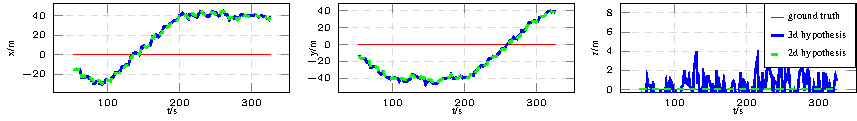
\includegraphics[width=1.0\textwidth]{./fig/plots/example_plot/hypotheses.pdf}
  \caption{Example of a 2D plot using \emph{PGFPlots}.}
  \label{fig:pgfplots_data}
\end{figure}

\section{3D Plots with Sketch}

\emph{Sketch} is a tool for defining a 3D scene using simple descriptive language.
The 3D scene is then converted to \emph{Tikz}, which is later compiled to pdf.
The benefits of using \emph{Sketch} are similar to using \emph{Tikz}: LaTeX fonts, versioning using git, and cleanness of the result.
See the example image in \reffig{fig:coordinate_systems}.
\begin{itemize}
  \item Documentation and manual: \url{http://www.frontiernet.net/~eugene.ressler/}
  \item Cross-compilation from \emph{Sketch} to \emph{pdf} using the \texttt{fig/sketch/compile\_sketch.sh} script.
\end{itemize}

\begin{figure}[htbp]
  \centering
  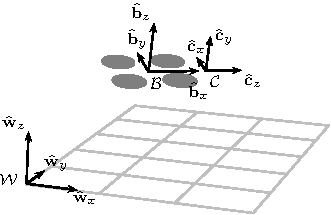
\includegraphics[width=0.4\textwidth]{./fig/sketch/coordinate_frames.pdf}
  \caption{Depiction of the used coordinate systems. The image was drawn using \emph{Sketch}.}
  \label{fig:coordinate_systems}
\end{figure}

\section{Image collages with Subfig}

We recommend using the \texttt{subfig} package, which provides the \texttt{\textbackslash{}subfloat} command.
It is more versatile than the simpler \texttt{subcaption} package.
Check \reffig{fig:uavs} for an example.

\begin{figure}[htbp]
  \centering
  \subfloat[A UAV, the T650 model.] {
    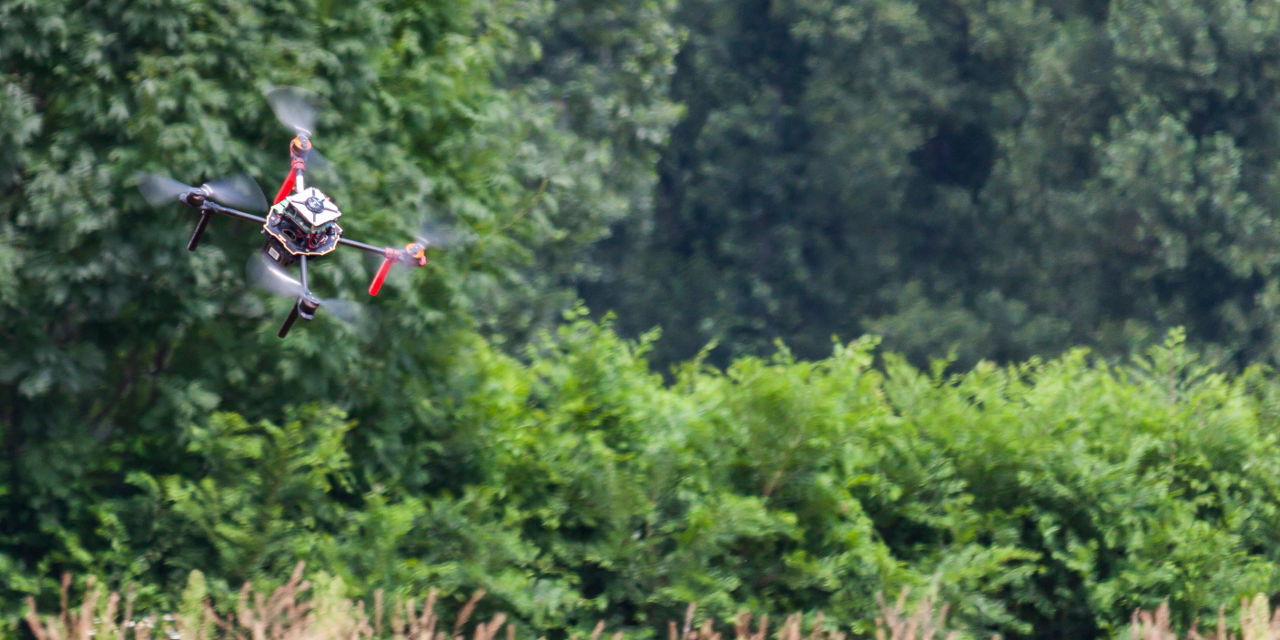
\includegraphics[width=0.48\textwidth]{./fig/photos/uav1.jpg}
    \label{fig:uavs_1}
  }
  \subfloat[Another UAV, again, the T650 model.] {
    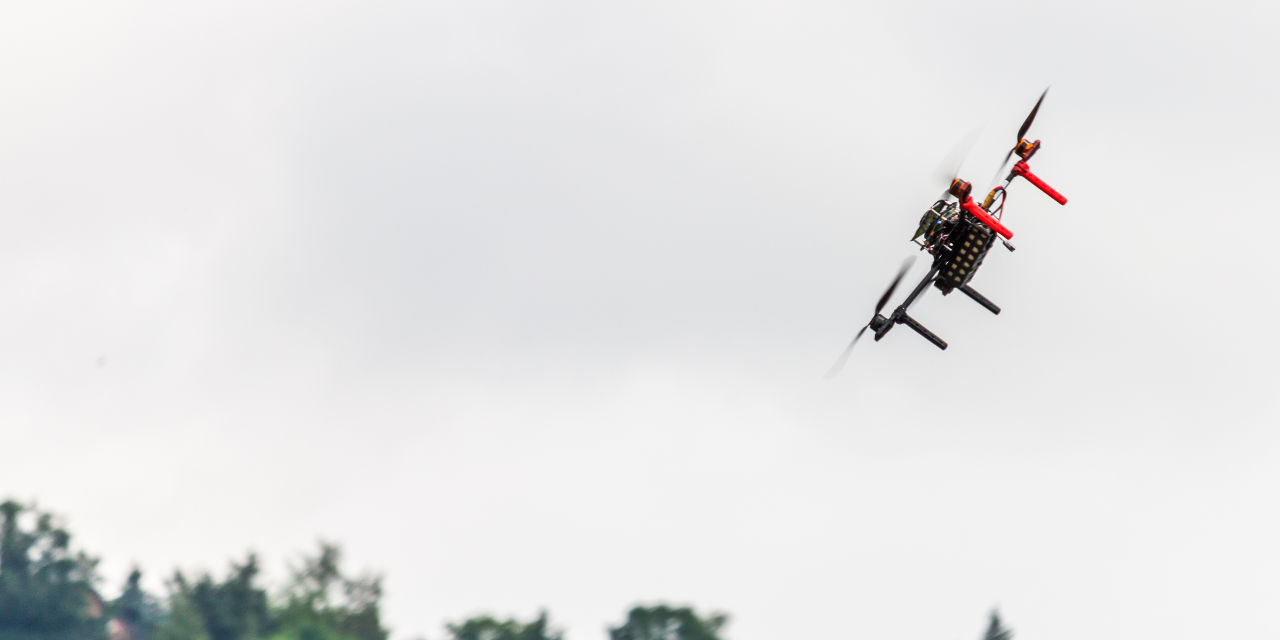
\includegraphics[width=0.48\textwidth]{./fig/photos/uav2.jpg}
    \label{fig:uavs_2}
  }
  \caption{
The caption should mention both subfigures, the \reffig{fig:uavs_1} and the \reffig{fig:uavs_2}.
You can just refer to them as (a) and (b) in the main Figure's caption, but beware, you need to keep it correct as you edit.
}
  \label{fig:uavs}
\end{figure}

\section{Citations with Biblatex}

\emph{Biblatex} is probably the most powerful citation package for LaTeX.
It consumes the standard \texttt{.bib} file. However, it can sort and filter the citations using the \texttt{keywords} tag.
Citing references is done using the \texttt{cite} command, e.g., \cite{baca2021mrs}.
You can also define some nice citation boxes, such as this one:
\fullciteinbox{baca2021mrs}{}

\section{Image overlays with Tikz}

\emph{Tikz} is very useful to create custom image overlays.
The overlay can be set such that the image is spanned by Cartesian coordinates $\left(x, y\right) \in \left[0, 1\right]^2$
Example can be seen in \reffig{fig:tikz_overlay}.

\begin{figure}[!t]

  \centering

  \subfloat {\begin{tikzpicture}
    \node[anchor=south west,inner sep=0] (a) at (0,0) { 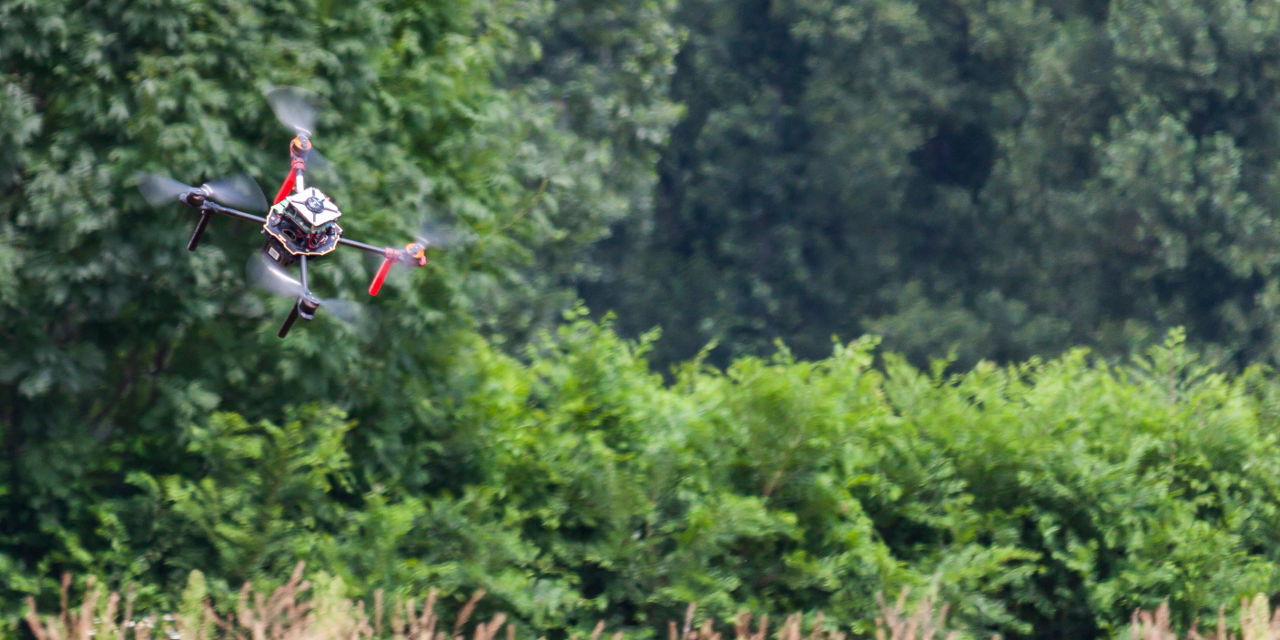
\includegraphics[width=0.45\textwidth]{./fig/photos/uav1.jpg}};
    \begin{scope}[x={(a.south east)},y={(a.north west)}]

      %%{ grid for placing the elements

      % % useful grid to help you find coordinates for plotting the overlay
      % \draw[black, xstep=.1, ystep=.1] (0,0) grid (1,1);
      % \foreach \i in {0,0.1,0.2,0.3,0.4,0.5,0.6,0.7,0.8,0.9,1} {
      %   \node[align=center] at (\i, -0.05) {\i};
      %   \node[align=center] at (\i, 1.05) {\i};
      %   \node[align=center] at (-0.05, \i) {\i};
      %   \node[align=center] at (1.05, \i) {\i};
      % }

      %%}

      % plot some stuff over the image

      % plot white background behind the letter (a)
      \fill[white] (0.001, 0.001) rectangle (0.08,0.14);

      % plot black border
      \fill[draw=black, draw opacity=0.5, fill opacity=0] (0,0) rectangle (1, 1);

      % write the letter (a) in the bottom-left corner
      \draw (0.04,0.06) node [text=black] {\small (a)};

      % plot black border
      \draw[->, white, thick] (0.50, 0.80) -- (0.30, 0.67);
      \draw (0.50,0.86) node [text=white] {\small \textbf{UAV}};
    \end{scope}
  \end{tikzpicture}}
\hfill%
\subfloat {\begin{tikzpicture}
    \node[anchor=south west,inner sep=0] (a) at (0,0) { 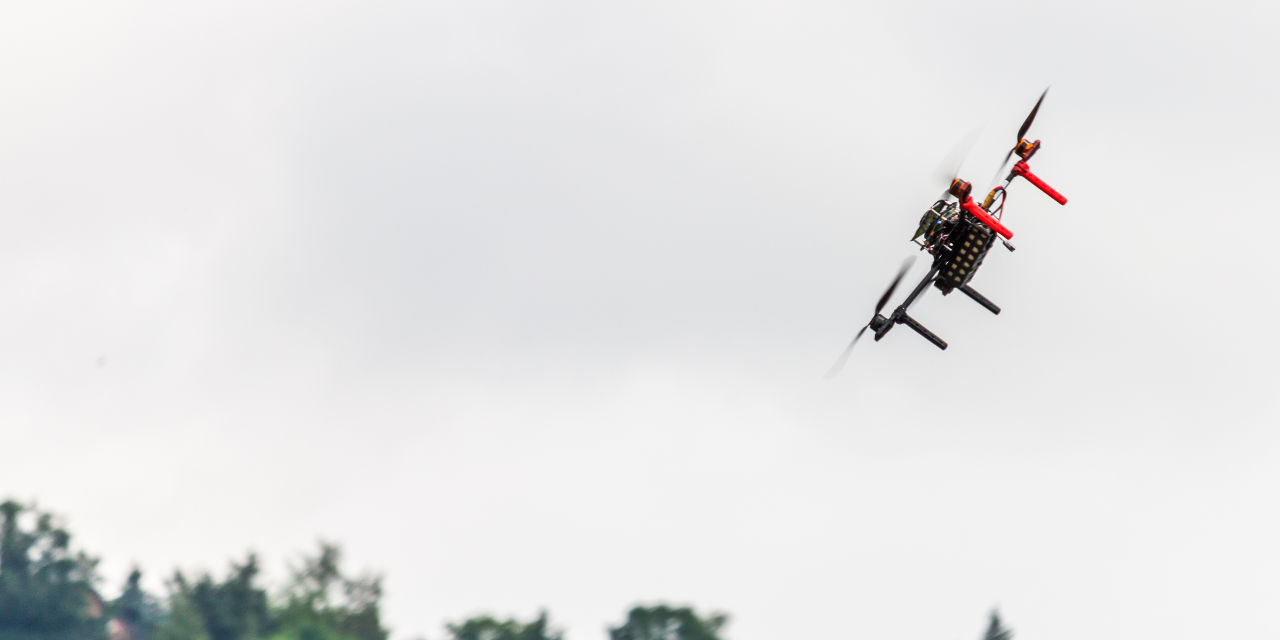
\includegraphics[width=0.45\textwidth]{./fig/photos/uav2.jpg}};
    \begin{scope}[x={(a.south east)},y={(a.north west)}]

      %%{ grid for placing the elements

      % useful grid to help you find coordinates for plotting the overlay
      \draw[black, xstep=.1, ystep=.1] (0,0) grid (1,1);
      \foreach \i in {0,0.1,0.2,0.3,0.4,0.5,0.6,0.7,0.8,0.9,1} {
        \node[align=center] at (\i, -0.05) {\i};
        \node[align=center] at (\i, 1.05) {\i};
        \node[align=center] at (-0.05, \i) {\i};
        \node[align=center] at (1.05, \i) {\i};
      }

      %%}

      % plot some stuff over the image

      % plot white background behind the letter (b)
      \fill[white] (0.001, 0.001) rectangle (0.08,0.14);

      % plot black border
      \fill[draw=black, draw opacity=0.5, fill opacity=0] (0,0) rectangle (1, 1);

      % write the letter (b) in the bottom-left corner
      \draw (0.04,0.06) node [text=black] {\small (b)};
    \end{scope}
  \end{tikzpicture}}


  \caption{Example of using Tikz for image overlays. (a) shows a final product, (b) shows a grid useful for nailing down the coordinates.}
  \label{fig:tikz_overlay}

\end{figure}

\section{General tips}

In general, strive to make the paper easy to read and understand, and hard to misunderstand or misinterpret.
Here are some more specific tips on how to achieve that (and other general suggestions).

\begin{itemize}
  \item
    \textbf{Be consistent.}
    This applies in all contexts.
    For example, if you decide to use the name \enquote{LiDAR}, do not mix it with \enquote{LIDAR} or \enquote{Lidar},
    do not mix different mathematical notations,
    ensure your Figures have the same style and use the same graphics for the same concepts,
    etc.
  \item 
    After you finish writing or modifying any of:
    \begin{itemize}
      \item a sentence,
      \item a paragraph,
      \item a section/chapter,
      \item the whole paper/thesis,
    \end{itemize}
    \textbf{re-read it} to make sure that it makes sense, it is coherent and correct, and doesn't contain typos.
  \item
    If you're using a LLM-based tool (ChatGPT etc.) for grammar-proofing or even formulation of sentences, \textbf{do not just copy-paste its response} to your query.
    The previous rule applies doubly here.
    LLMs tend to often produce confident-sounding nonsense, sentences with reformulated duplicated content, or with a slightly changed meaning.
    They are a good tool to get inspiration to start writing about a subject, for grammar-checking, or for finding alternative, nice-sounding formulations, but they can lie or warp facts --- take care when using them!

\end{itemize}


%% --------------------------------------------------------------
%% |                         Conclusion                         |
%% --------------------------------------------------------------

%!TEX root = ../main.tex

\chapter{Conclusion\label{chap:conclusion}}

This thesis set out to address key challenges in autonomous \ac{UAV} operations. 
The work focused on two primary objectives: first, to extend the established two-dimensional \ac{RBL} algorithm for effective multi-agent coordination in three-dimensional space, introducing new rules to enhance its performance. 
Secondly validating the practical application of this extended framework for single  \ac{UAV} navigation in a complex, GNSS-denied forest environment using onboard \ac{LiDAR} sensing.

The core contributions of this work began with the successful extension of the \ac{RBL} algorithm to 3D. 
This involved key modifications such as adapting Voronoi cell partitioning for three dimensions, modifying existing rules, and introducing a new elevation rotation angle designed to adjust the agent's vertical destination and improve spatial distribution. 
Simulations of multi-agent scenarios, including crossing circle and sphere formations, demonstrated that these extensions successfully enabled coordination in three dimensions. 
Notably, analysis revealed a trend where the performance advantage of the 3D \ac{RBL} approach with these rules, compared to the basic 2D version, increased with the number of agents.

Building upon this, the second major contribution was the practical implementation and real-world validation of the 3D \ac{RBL} algorithm for single  \ac{UAV} navigation. 
This involved integrating the algorithm with \ac{LiDAR}-based perception, Point-LIO for state estimation, and the Bonxai voxel-based mapping. 
Key technical advancements included adapting the \ac{RBL} cell partitioning to directly utilize voxelized map data and implementing software modifications to effectively handle the practical limitations of a single \ac{LiDAR} sensor with a restricted vertical field of view, ensuring safe movement based on actively sensed areas while still leveraging map information. 
Real-world experiments in a forest environment successfully demonstrated the  \ac{UAV}'s ability to navigate autonomously between designated start and goal points, avoiding static obstacles like trees and adapting its altitude based on \ac{LiDAR} perception, as shown in the provided flight videos \cite{aggressive_flight}, \cite{conservative_flight}.

The significance of these findings lies in advancing decentralized, rule-based control strategies for \ac{UAV}s operating in three dimensions. 
The successful 3D extension of \ac{RBL} offers a scalable approach for multi-agent systems, while the demonstration of \ac{LiDAR}-based navigation in a real forest highlights the potential for autonomous operations in GPS-denied settings. 

However, the research also identified limitations. 
For the multi-agent 3D \ac{RBL}, while simulations indicated advantages, the degree of improvement was occasionally less noticeable, possibly a result of conservative motion constraints and parameter settings that could be refined through further tuning.
The algorithm also requires an initial shared frame of reference for certain directional rules to function optimally. 
In the single-agent forest navigation, the primary challenge encountered was Bonxai mapping package, particularly its handling of dynamic environmental elements like moving leaves, which occasionally led to navigation deadlocks \cite{flight_fail}. 
This highlights the dependence of the current navigation approach on an accurate map representation.

Future work should therefore focus on improving the system's ability to handle dynamic obstacles. 
This could involve implementing another mapping algorithm or more sophisticated map update and filtering techniques, or by developing strategies that allow the UAV to react more directly to sensor perceptions of the environment, reducing dependence on map.

In conclusion, this thesis has successfully demonstrated the extension of the \ac{RBL} algorithm to 3D for multi-agent coordination in simulation and its practical application for single \ac{UAV} navigation in a real-world environment using \ac{LiDAR}. 
While challenges, particularly in perception and mapping in dynamic settings, remain, the presented work provides a valuable contribution and a solid foundation for future advancements in autonomous, rule-based \ac{UAV} navigation and coordination.


%% --------------------------------------------------------------
%% |                         References                         |
%% --------------------------------------------------------------

\chapter{References}

\printbibliography[heading=none,title={}]

%% --------------------------------------------------------------
%% |                         Appendices                         |
%% --------------------------------------------------------------

\appendix
\renewcommand\chaptername{Appendix}

\renewcommand{\thechapter}{A}
\renewcommand\chaptername{Appendix A}

\chapter{Appendix A}

\end{document}
